% Options for packages loaded elsewhere
\PassOptionsToPackage{unicode}{hyperref}
\PassOptionsToPackage{hyphens}{url}
%
\documentclass[
]{article}
\usepackage{lmodern}
\usepackage{amssymb,amsmath}
\usepackage{ifxetex,ifluatex}
\ifnum 0\ifxetex 1\fi\ifluatex 1\fi=0 % if pdftex
  \usepackage[T1]{fontenc}
  \usepackage[utf8]{inputenc}
  \usepackage{textcomp} % provide euro and other symbols
\else % if luatex or xetex
  \usepackage{unicode-math}
  \defaultfontfeatures{Scale=MatchLowercase}
  \defaultfontfeatures[\rmfamily]{Ligatures=TeX,Scale=1}
\fi
% Use upquote if available, for straight quotes in verbatim environments
\IfFileExists{upquote.sty}{\usepackage{upquote}}{}
\IfFileExists{microtype.sty}{% use microtype if available
  \usepackage[]{microtype}
  \UseMicrotypeSet[protrusion]{basicmath} % disable protrusion for tt fonts
}{}
\makeatletter
\@ifundefined{KOMAClassName}{% if non-KOMA class
  \IfFileExists{parskip.sty}{%
    \usepackage{parskip}
  }{% else
    \setlength{\parindent}{0pt}
    \setlength{\parskip}{6pt plus 2pt minus 1pt}}
}{% if KOMA class
  \KOMAoptions{parskip=half}}
\makeatother
\usepackage{xcolor}
\IfFileExists{xurl.sty}{\usepackage{xurl}}{} % add URL line breaks if available
\IfFileExists{bookmark.sty}{\usepackage{bookmark}}{\usepackage{hyperref}}
\hypersetup{
  pdftitle={MATH501 Coursework - Report},
  pdfauthor={10570155, 10696253, 10701983},
  hidelinks,
  pdfcreator={LaTeX via pandoc}}
\urlstyle{same} % disable monospaced font for URLs
\usepackage[margin=1in]{geometry}
\usepackage{color}
\usepackage{fancyvrb}
\newcommand{\VerbBar}{|}
\newcommand{\VERB}{\Verb[commandchars=\\\{\}]}
\DefineVerbatimEnvironment{Highlighting}{Verbatim}{commandchars=\\\{\}}
% Add ',fontsize=\small' for more characters per line
\usepackage{framed}
\definecolor{shadecolor}{RGB}{248,248,248}
\newenvironment{Shaded}{\begin{snugshade}}{\end{snugshade}}
\newcommand{\AlertTok}[1]{\textcolor[rgb]{0.94,0.16,0.16}{#1}}
\newcommand{\AnnotationTok}[1]{\textcolor[rgb]{0.56,0.35,0.01}{\textbf{\textit{#1}}}}
\newcommand{\AttributeTok}[1]{\textcolor[rgb]{0.77,0.63,0.00}{#1}}
\newcommand{\BaseNTok}[1]{\textcolor[rgb]{0.00,0.00,0.81}{#1}}
\newcommand{\BuiltInTok}[1]{#1}
\newcommand{\CharTok}[1]{\textcolor[rgb]{0.31,0.60,0.02}{#1}}
\newcommand{\CommentTok}[1]{\textcolor[rgb]{0.56,0.35,0.01}{\textit{#1}}}
\newcommand{\CommentVarTok}[1]{\textcolor[rgb]{0.56,0.35,0.01}{\textbf{\textit{#1}}}}
\newcommand{\ConstantTok}[1]{\textcolor[rgb]{0.00,0.00,0.00}{#1}}
\newcommand{\ControlFlowTok}[1]{\textcolor[rgb]{0.13,0.29,0.53}{\textbf{#1}}}
\newcommand{\DataTypeTok}[1]{\textcolor[rgb]{0.13,0.29,0.53}{#1}}
\newcommand{\DecValTok}[1]{\textcolor[rgb]{0.00,0.00,0.81}{#1}}
\newcommand{\DocumentationTok}[1]{\textcolor[rgb]{0.56,0.35,0.01}{\textbf{\textit{#1}}}}
\newcommand{\ErrorTok}[1]{\textcolor[rgb]{0.64,0.00,0.00}{\textbf{#1}}}
\newcommand{\ExtensionTok}[1]{#1}
\newcommand{\FloatTok}[1]{\textcolor[rgb]{0.00,0.00,0.81}{#1}}
\newcommand{\FunctionTok}[1]{\textcolor[rgb]{0.00,0.00,0.00}{#1}}
\newcommand{\ImportTok}[1]{#1}
\newcommand{\InformationTok}[1]{\textcolor[rgb]{0.56,0.35,0.01}{\textbf{\textit{#1}}}}
\newcommand{\KeywordTok}[1]{\textcolor[rgb]{0.13,0.29,0.53}{\textbf{#1}}}
\newcommand{\NormalTok}[1]{#1}
\newcommand{\OperatorTok}[1]{\textcolor[rgb]{0.81,0.36,0.00}{\textbf{#1}}}
\newcommand{\OtherTok}[1]{\textcolor[rgb]{0.56,0.35,0.01}{#1}}
\newcommand{\PreprocessorTok}[1]{\textcolor[rgb]{0.56,0.35,0.01}{\textit{#1}}}
\newcommand{\RegionMarkerTok}[1]{#1}
\newcommand{\SpecialCharTok}[1]{\textcolor[rgb]{0.00,0.00,0.00}{#1}}
\newcommand{\SpecialStringTok}[1]{\textcolor[rgb]{0.31,0.60,0.02}{#1}}
\newcommand{\StringTok}[1]{\textcolor[rgb]{0.31,0.60,0.02}{#1}}
\newcommand{\VariableTok}[1]{\textcolor[rgb]{0.00,0.00,0.00}{#1}}
\newcommand{\VerbatimStringTok}[1]{\textcolor[rgb]{0.31,0.60,0.02}{#1}}
\newcommand{\WarningTok}[1]{\textcolor[rgb]{0.56,0.35,0.01}{\textbf{\textit{#1}}}}
\usepackage{graphicx,grffile}
\makeatletter
\def\maxwidth{\ifdim\Gin@nat@width>\linewidth\linewidth\else\Gin@nat@width\fi}
\def\maxheight{\ifdim\Gin@nat@height>\textheight\textheight\else\Gin@nat@height\fi}
\makeatother
% Scale images if necessary, so that they will not overflow the page
% margins by default, and it is still possible to overwrite the defaults
% using explicit options in \includegraphics[width, height, ...]{}
\setkeys{Gin}{width=\maxwidth,height=\maxheight,keepaspectratio}
% Set default figure placement to htbp
\makeatletter
\def\fps@figure{htbp}
\makeatother
\setlength{\emergencystretch}{3em} % prevent overfull lines
\providecommand{\tightlist}{%
  \setlength{\itemsep}{0pt}\setlength{\parskip}{0pt}}
\setcounter{secnumdepth}{-\maxdimen} % remove section numbering

\title{MATH501 Coursework - Report}
\author{10570155, 10696253, 10701983}
\date{26/04/2021}

\begin{document}
\maketitle

The following report will discuss the results of the MATH501 questions
that were asked in two sections of machine learning and statistical
analysis.

\hypertarget{machine-learning}{%
\section{Machine Learning}\label{machine-learning}}

\hypertarget{part-a}{%
\subsection{Part (a)}\label{part-a}}

\textbf{Present the data visually using box-and-whisker plots with a
distinction for churn. Comment on the data in the context of the
problem.}

Reading our data in a dataframe:

\begin{Shaded}
\begin{Highlighting}[]
\NormalTok{data_path <-}\StringTok{ "data/churndata.txt"}
\NormalTok{churn_data <-}\StringTok{ }\KeywordTok{read.csv}\NormalTok{(data_path, }\DataTypeTok{sep =} \StringTok{" "}\NormalTok{)}
\NormalTok{churn_data <-}\StringTok{ }\KeywordTok{na.exclude}\NormalTok{(churn_data) }\CommentTok{# removing entries with NA values}
\CommentTok{# converting classifier to a factor:}
\NormalTok{churn_data}\OperatorTok{$}\NormalTok{churn <-}\StringTok{ }\KeywordTok{as.factor}\NormalTok{(churn_data}\OperatorTok{$}\NormalTok{churn) }
\end{Highlighting}
\end{Shaded}

The data includes 4 predictors - `webget', `callwait', `upload' and
`enqcount' and a classifier `churn' which identifies whether a client
has switched to a new operator or not.

\begin{Shaded}
\begin{Highlighting}[]
\KeywordTok{head}\NormalTok{(churn_data)}
\end{Highlighting}
\end{Shaded}

\begin{verbatim}
##   upload webget enqcount callwait churn
## 1    9.2  283.9        5     8.14    no
## 2    7.0  298.4        6    11.59    no
## 3    6.6  163.8        5     8.25    no
## 4   15.0  566.8        2     9.50    no
## 5   11.1  210.3        5     6.96    no
## 6   15.4  857.0        2    10.80   yes
\end{verbatim}

Boxplot with average speed of upload against an indicator whether a
customer switched to a different provider:

\begin{Shaded}
\begin{Highlighting}[]
\NormalTok{churn_data }\OperatorTok\StringTok{ }\KeywordTok{ggplot}\NormalTok{(}\KeywordTok{aes}\NormalTok{(}\DataTypeTok{x =}\NormalTok{ churn, }\DataTypeTok{y =}\NormalTok{ upload, }\DataTypeTok{color =}\NormalTok{ churn)) }\OperatorTok{+}\StringTok{ }
\StringTok{ }\KeywordTok{geom_boxplot}\NormalTok{() }\OperatorTok{+}
\StringTok{ }\KeywordTok{labs}\NormalTok{ (}\DataTypeTok{y =} \StringTok{"Speed of upload"}\NormalTok{, }
       \DataTypeTok{x =} \StringTok{"Switched to a new provider"}\NormalTok{,}
       \DataTypeTok{color =} \StringTok{"Switched"}\NormalTok{)}
\end{Highlighting}
\end{Shaded}

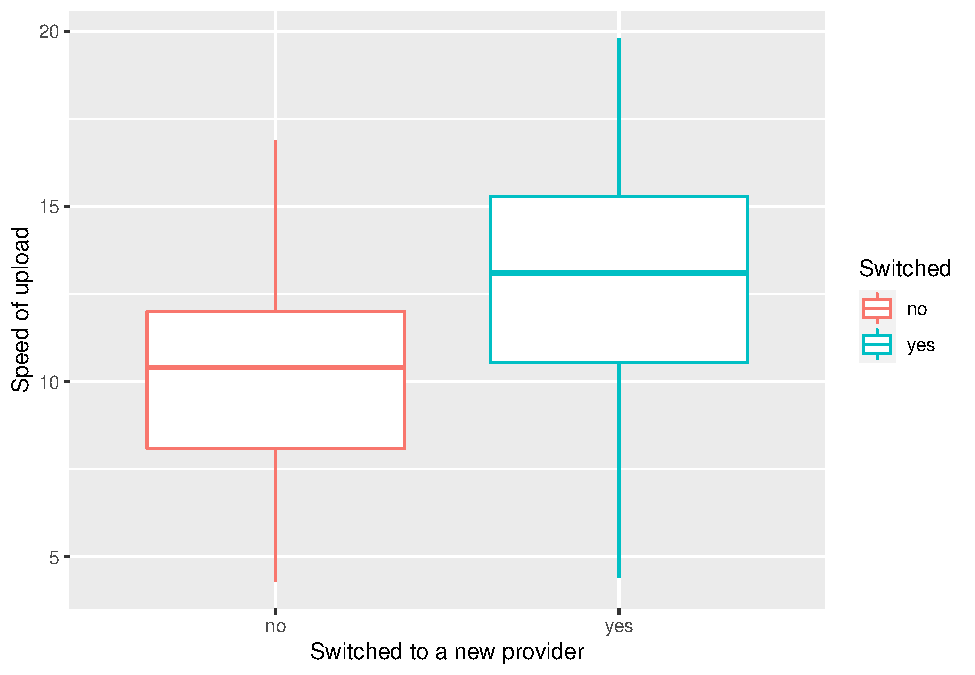
\includegraphics{Report_files/figure-latex/unnamed-chunk-2-1.pdf}

As we can see the customers who have not yet switched to a different
operator have lower average speed of upload in the internet in
comparison with the customers who have switched. In general, having
higher uplink speed is a plus since it improves the Internet phone/video
call experience and it does no harm to the customers Hence increasing
uplink speed could not affect the customers' decision to switch to
different operators.

Boxplot with the mean time to load a webpage against an indicator
whether a customer switched to a different provider:

\begin{Shaded}
\begin{Highlighting}[]
\NormalTok{churn_data }\OperatorTok\StringTok{ }\KeywordTok{ggplot}\NormalTok{(}\KeywordTok{aes}\NormalTok{(}\DataTypeTok{x =}\NormalTok{ churn, }\DataTypeTok{y =}\NormalTok{ webget, }\DataTypeTok{color =}\NormalTok{ churn)) }\OperatorTok{+}\StringTok{ }
\StringTok{ }\KeywordTok{geom_boxplot}\NormalTok{() }\OperatorTok{+}
\StringTok{ }\KeywordTok{labs}\NormalTok{ (}\DataTypeTok{y =} \StringTok{"Average time to load a webpage"}\NormalTok{, }
       \DataTypeTok{x =} \StringTok{"Switched to a new provider"}\NormalTok{,}
       \DataTypeTok{color =} \StringTok{"Switched"}\NormalTok{)}
\end{Highlighting}
\end{Shaded}

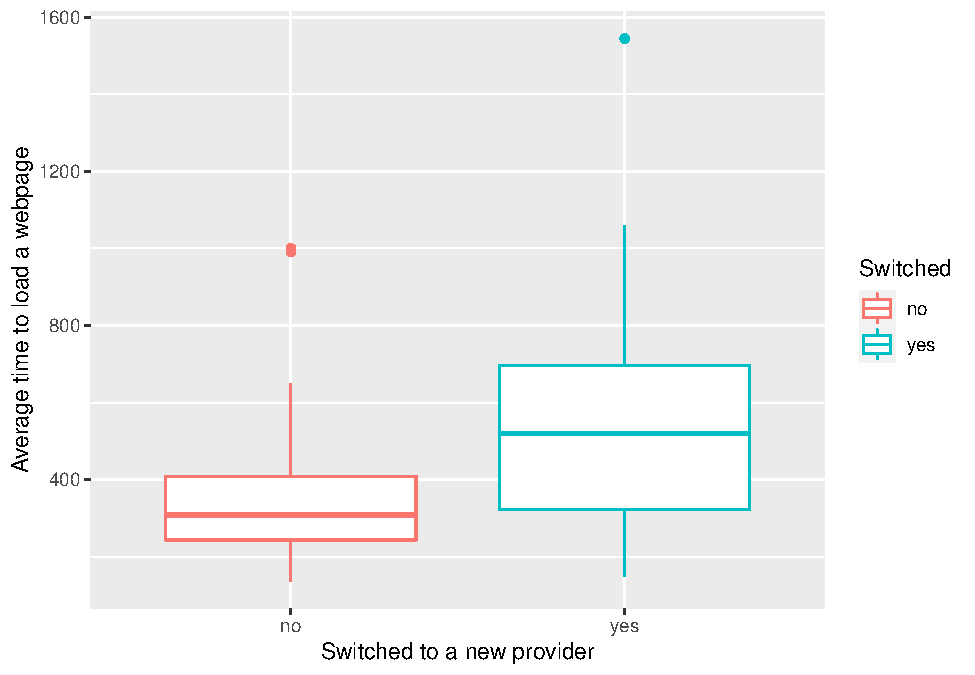
\includegraphics{Report_files/figure-latex/unnamed-chunk-3-1.pdf}

We can observe a strong dependency between the time to load a webpage
(which directly corresponds to the downlink speed) and an indicator
whether customers changed their operators. The average downlink speed
was significantly lower for the customers that have switched to a
different provider than for those who haven't. We can conclude this as
the average time to load a webpage for those clients who switched is
nearly 200 units longer than of those who didn't.

Boxplot with how long a customer waited on the phone call for a customer
service operator against an indicator whether a customer switched to a
different provider:

\begin{Shaded}
\begin{Highlighting}[]
\NormalTok{churn_data }\OperatorTok\StringTok{ }\KeywordTok{ggplot}\NormalTok{(}\KeywordTok{aes}\NormalTok{(}\DataTypeTok{x =}\NormalTok{ churn, }\DataTypeTok{y =}\NormalTok{ callwait, }\DataTypeTok{color =}\NormalTok{ churn)) }\OperatorTok{+}\StringTok{ }
\StringTok{ }\KeywordTok{geom_boxplot}\NormalTok{() }\OperatorTok{+}
\StringTok{ }\KeywordTok{labs}\NormalTok{ (}\DataTypeTok{y =} \StringTok{"Customer service waiting time"}\NormalTok{, }
       \DataTypeTok{x =} \StringTok{"Switched to a new provider"}\NormalTok{,}
       \DataTypeTok{color =} \StringTok{"Switched"}\NormalTok{)}
\end{Highlighting}
\end{Shaded}

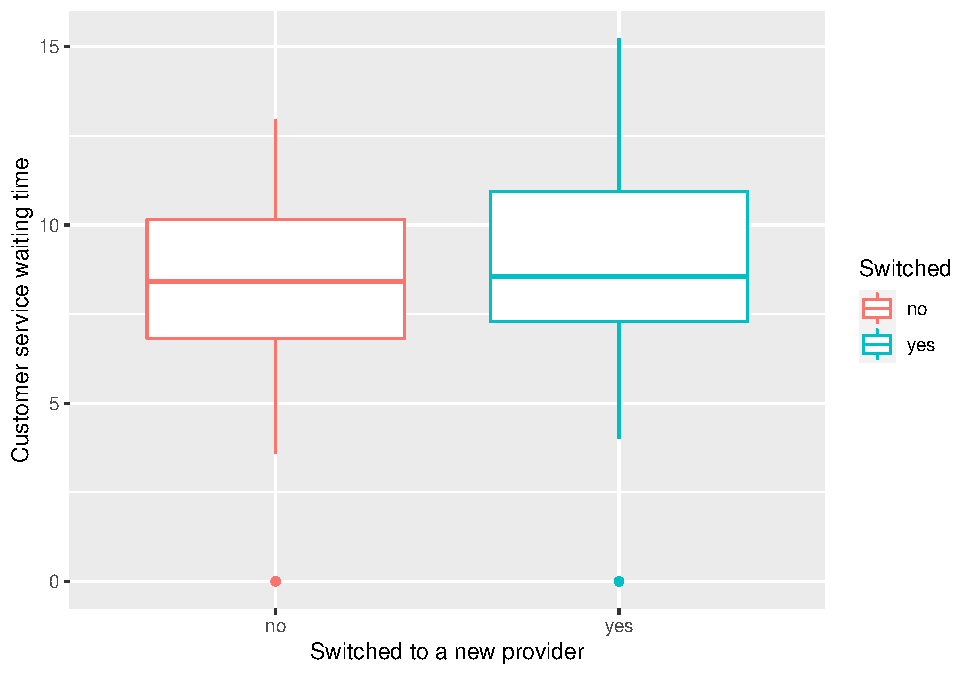
\includegraphics{Report_files/figure-latex/unnamed-chunk-4-1.pdf}

Even though the average waiting time for a customer service operator is
similar in both cases, overall the majority of of customers who switched
to a different operator had to wait longer than the average and the
customers who haven't changed their provider. We can assume that the
time spent by a customer on a call while they're waiting for a customer
service operator to attend may impact their decision to switch to
another operator although the influence seems to be less significant
compared to time to load a webpage.

Boxplot with the number of times a customer contacted the company via a
phone call against an indicator whether a customer switched to a
different provider:

\begin{Shaded}
\begin{Highlighting}[]
\NormalTok{churn_data }\OperatorTok\StringTok{ }\KeywordTok{ggplot}\NormalTok{(}\KeywordTok{aes}\NormalTok{(}\DataTypeTok{x =}\NormalTok{ churn, }\DataTypeTok{y =}\NormalTok{ enqcount, }\DataTypeTok{color =}\NormalTok{ churn)) }\OperatorTok{+}\StringTok{ }
\StringTok{ }\KeywordTok{geom_boxplot}\NormalTok{() }\OperatorTok{+}
\StringTok{ }\KeywordTok{labs}\NormalTok{ (}\DataTypeTok{y =} \StringTok{"The number of times a customer contacted the company"}\NormalTok{, }
       \DataTypeTok{x =} \StringTok{"Switched to a new provider"}\NormalTok{,}
       \DataTypeTok{color =} \StringTok{"Switched"}\NormalTok{)}
\end{Highlighting}
\end{Shaded}

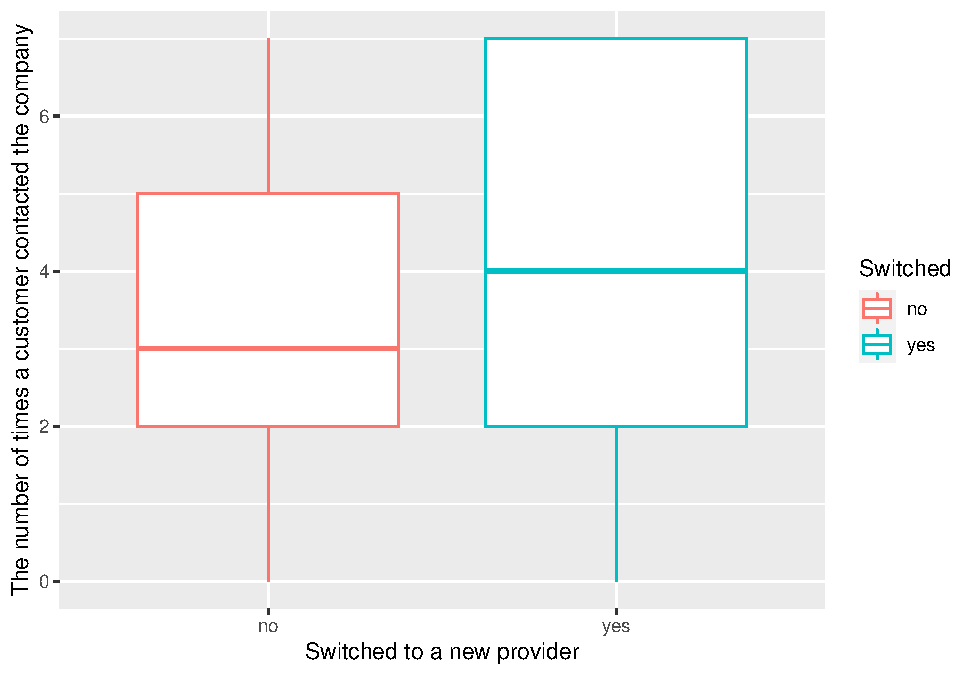
\includegraphics{Report_files/figure-latex/unnamed-chunk-5-1.pdf}

We can observe that in average the customers that switched to a
different operator contacted the company via a phone call 1 time more
often than others The biggest number of contact attempts is 2 calls more
than of the customers who haven't changed their providers. Needs to be
mentioned that some of the customers who switched didn't contact the
company even once. On the contrary minority of the customers who haven't
changed their provider also have more than 5 and even 6 calls. Still it
will be safe to assume that the number of calls impacts the customers'
decision to choose a different operator but its importance is smaller
the time to load a webpage.

\textbf{Conclusion}

Out of all the 4 factors that can possibly influence the `churn'
variable time to load the webpage (which subsequently leads to the
downlink speed) is the most important one. Average phone call customer
service waiting time doesn't differ drastically but still is higher for
customers who chose different providers hence we could conclude that
this aspect also plays its part in the customers' decision as well as
the number of phone calls to the company. The most suspicious variable
is the upload speed - for those clients who changed their providers the
uplink speed was actually higher but the downlink speed was lower
(comparing to the customers who didn't change their provider) while
normaly the opposite should be the case (unless we're talking about 5G).
Unfortunately, we don't have access to any other data hence we can only
speculate that perhaps there are some issues with the provider's
network.

\hypertarget{part-b}{%
\subsection{\texorpdfstring{\textbf{Part (b)}}{Part (b)}}\label{part-b}}

\textbf{Create a training set consisting of 350 randomly chosen data
points and a test set consisting of the remaining 150 data points.}

\begin{Shaded}
\begin{Highlighting}[]
\KeywordTok{set.seed}\NormalTok{(}\DecValTok{1}\NormalTok{) }\CommentTok{# to make the results reproducible}
\NormalTok{num_subset <-}\StringTok{ }\KeywordTok{sample}\NormalTok{(}\KeywordTok{nrow}\NormalTok{(churn_data), }\DecValTok{350}\NormalTok{) }\CommentTok{# randomly choose 350 numbers out of 500}
\end{Highlighting}
\end{Shaded}

Separating the data into predictors (X) and classifier (Y):

\begin{Shaded}
\begin{Highlighting}[]
\KeywordTok{attach}\NormalTok{(churn_data)}

\NormalTok{X <-}\StringTok{ }\KeywordTok{cbind}\NormalTok{(upload, webget, enqcount, callwait) }
\NormalTok{Y <-}\StringTok{ }\NormalTok{churn}
\NormalTok{Y <-}\StringTok{ }\KeywordTok{as.integer}\NormalTok{(Y }\OperatorTok{==}\StringTok{ 'yes'}\NormalTok{)}
\NormalTok{Y <-}\StringTok{ }\KeywordTok{as.factor}\NormalTok{(Y)}

\KeywordTok{detach}\NormalTok{(churn_data)}
\end{Highlighting}
\end{Shaded}

Dividing the data into training and testing sets:

\begin{Shaded}
\begin{Highlighting}[]
\NormalTok{train.X <-}\StringTok{ }\NormalTok{X[num_subset, ] }\CommentTok{# 350 records}
\NormalTok{train.Y <-}\StringTok{ }\NormalTok{Y[num_subset]}

\NormalTok{test.X <-}\StringTok{ }\NormalTok{X[}\OperatorTok{-}\NormalTok{num_subset, ] }\CommentTok{# 150 records}
\NormalTok{test.Y <-}\StringTok{ }\NormalTok{Y[}\OperatorTok{-}\NormalTok{num_subset]}
\end{Highlighting}
\end{Shaded}

\hypertarget{part-c}{%
\subsection{\texorpdfstring{\textbf{Part (c)}}{Part (c)}}\label{part-c}}

\textbf{Using the training data set apply the K nearest neighbours
method to construct a classifier to predict churn based on the four
available predictors. Find the optimal K using leave-one-out
cross-validation for the training data set. Calculate the test error for
the classification rule obtained for the optimal K.}

Before actually applying KNN we need to normalise the dataset because
our data has different units and is on a different scale.

Writing a function for normalising our predictors: substracting mean
value and diving the result by the standard deviation.

\begin{Shaded}
\begin{Highlighting}[]
\NormalTok{normalise <-}\StringTok{ }\ControlFlowTok{function}\NormalTok{ (inList)\{}
\NormalTok{  m <-}\StringTok{ }\KeywordTok{mean}\NormalTok{(inList)}
\NormalTok{  s <-}\StringTok{ }\KeywordTok{sd}\NormalTok{(inList)}
\NormalTok{  inList <-}\StringTok{ }\NormalTok{(inList }\OperatorTok{-}\StringTok{ }\NormalTok{m)}\OperatorTok{/}\NormalTok{s}
  \KeywordTok{return}\NormalTok{(inList)}
\NormalTok{\}}
\end{Highlighting}
\end{Shaded}

Applying this function to each of the columns in our test and traininig
sets:

\begin{Shaded}
\begin{Highlighting}[]
\NormalTok{train.X <-}\StringTok{ }\KeywordTok{apply}\NormalTok{(train.X, }\DecValTok{2}\NormalTok{, normalise)}
\NormalTok{test.X <-}\StringTok{ }\KeywordTok{apply}\NormalTok{(test.X, }\DecValTok{2}\NormalTok{, normalise)}
\end{Highlighting}
\end{Shaded}

Now our predictors have values in the same range.

\begin{Shaded}
\begin{Highlighting}[]
\KeywordTok{head}\NormalTok{(train.X)}
\end{Highlighting}
\end{Shaded}

\begin{verbatim}
##          upload     webget   enqcount   callwait
## [1,]  0.9790438  1.5490048 -0.6603278 -0.2912318
## [2,] -1.0678586 -0.7647049  1.7222982 -0.7052967
## [3,] -0.9637788 -1.0506624 -0.6603278  0.5692468
## [4,]  0.2851786 -0.6131415 -0.6603278 -0.1391924
## [5,] -1.4841777 -1.2034098 -0.1838026  0.2878121
## [6,]  0.2851786 -0.3704033  0.7692478  1.4167860
\end{verbatim}

Writing a function for KNN with leave-one-out cross-validation.
Leave-one-out is a special case of k-fold cross validation.

\begin{Shaded}
\begin{Highlighting}[]
\NormalTok{leave.KNN <-}\StringTok{ }\ControlFlowTok{function}\NormalTok{(K, train.X, train.Y)\{}
\NormalTok{  error <-}\StringTok{ }\DecValTok{0}
\NormalTok{  n <-}\StringTok{ }\KeywordTok{nrow}\NormalTok{(train.X)}
  \CommentTok{# this function returns an error that is calculated as an average error of KNNs trained }
  \CommentTok{# using leave-one-out}
        \ControlFlowTok{for}\NormalTok{(i }\ControlFlowTok{in} \DecValTok{1}\OperatorTok{:}\NormalTok{n)\{}
          \CommentTok{# subsetting the i-th row from the train predictors and classifiers and using}
          \CommentTok{# them as temporary training sets (without an i-th row)}
\NormalTok{          temp.train.X <-}\StringTok{ }\NormalTok{train.X[}\OperatorTok{-}\NormalTok{i,]}
\NormalTok{          temp.train.Y <-}\StringTok{ }\NormalTok{train.Y[}\OperatorTok{-}\NormalTok{i]}

          \CommentTok{# using an i-th row as a temporary test set}
\NormalTok{          temp.test.X <-}\StringTok{ }\NormalTok{train.X[i,]}
\NormalTok{          temp.test.Y <-}\StringTok{ }\NormalTok{train.Y[i]}

          \CommentTok{# the resulting KNN is tested on only 1 entry}
\NormalTok{          temp.knn <-}\StringTok{ }\KeywordTok{knn}\NormalTok{(}
            \DataTypeTok{train =}\NormalTok{ temp.train.X, }
            \DataTypeTok{test =}\NormalTok{ temp.test.X, }
            \DataTypeTok{cl =}\NormalTok{ temp.train.Y, }\DataTypeTok{k =}\NormalTok{ K)}

          \CommentTok{# the error is being calculated on whether a test entry was classified wrongly }
          \CommentTok{# or not and accumulated as we'll need to find the mean error in the end}
\NormalTok{          error <-}\StringTok{ }\NormalTok{error }\OperatorTok{+}\StringTok{ }\KeywordTok{mean}\NormalTok{(temp.knn }\OperatorTok{!=}\StringTok{ }\NormalTok{temp.test.Y) }
            \CommentTok{# 1 if the test entry was classified wrongly and 0 if correctly}
\NormalTok{        \}}

     \KeywordTok{return}\NormalTok{ (error}\OperatorTok{/}\NormalTok{n) }\CommentTok{#returning the average error}
\NormalTok{\}}
\end{Highlighting}
\end{Shaded}

Now trying to find the optimal K in a range of values between 1 to 30.
Running the \emph{leave.KNN} function in a loop and storing the
calculated in the function error in an array.

\begin{Shaded}
\begin{Highlighting}[]
\NormalTok{errors <-}\StringTok{ }\KeywordTok{rep}\NormalTok{(}\DecValTok{0}\NormalTok{, }\DecValTok{30}\NormalTok{) }\CommentTok{#trying with K from 1 to 30}
\ControlFlowTok{for}\NormalTok{ (j }\ControlFlowTok{in} \DecValTok{1}\OperatorTok{:}\DecValTok{30}\NormalTok{) errors[j] <-}\StringTok{ }\KeywordTok{leave.KNN}\NormalTok{(j, train.X, train.Y)}
\end{Highlighting}
\end{Shaded}

Plotting our errors

\begin{Shaded}
\begin{Highlighting}[]
\CommentTok{# plotting errors}
\KeywordTok{plot}\NormalTok{(errors, }\DataTypeTok{xlab=}\StringTok{"K"}\NormalTok{, }\DataTypeTok{ylab =} \StringTok{"Test error"}\NormalTok{)}
\end{Highlighting}
\end{Shaded}

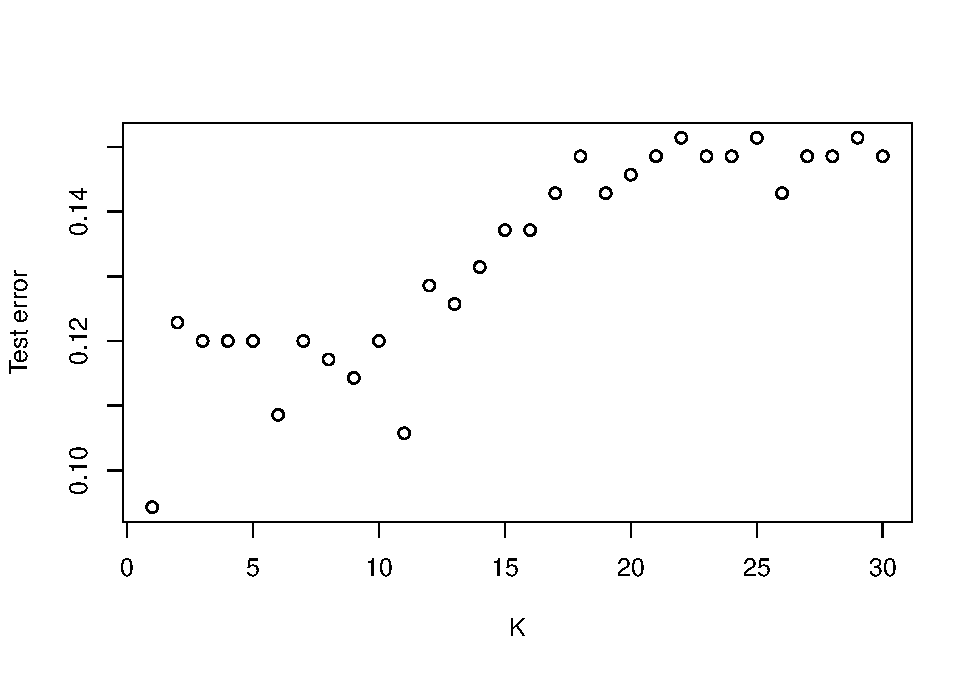
\includegraphics{Report_files/figure-latex/unnamed-chunk-14-1.pdf}

Finding optimal K as an index of the first smallest error value

\begin{Shaded}
\begin{Highlighting}[]
\NormalTok{optim.K <-}\StringTok{ }\KeywordTok{which.min}\NormalTok{(errors)}
\end{Highlighting}
\end{Shaded}

Now running KNN with the optimal K found from the leave-one-out
cross-validation.

\begin{Shaded}
\begin{Highlighting}[]
\NormalTok{def.knn <-}\StringTok{ }\KeywordTok{knn}\NormalTok{(}\DataTypeTok{train =}\NormalTok{ train.X, }\DataTypeTok{test =}\NormalTok{ test.X, }\DataTypeTok{cl =}\NormalTok{ train.Y, }\DataTypeTok{k =}\NormalTok{ optim.K) }\CommentTok{# yep that's it}
\NormalTok{tab <-}\StringTok{ }\KeywordTok{table}\NormalTok{(def.knn, test.Y) }\CommentTok{# confusion table}
\end{Highlighting}
\end{Shaded}

Calculating the error using falsely predicted churn values

\begin{Shaded}
\begin{Highlighting}[]
\NormalTok{error.KNN <-}\StringTok{ }\NormalTok{(tab[}\DecValTok{1}\NormalTok{,}\DecValTok{2}\NormalTok{] }\OperatorTok{+}\StringTok{ }\NormalTok{tab[}\DecValTok{2}\NormalTok{,}\DecValTok{1}\NormalTok{]) }\OperatorTok{/}\StringTok{ }\KeywordTok{sum}\NormalTok{(tab) }
\KeywordTok{sprintf}\NormalTok{(}\StringTok{"Expected error: %f Test error: %f"}\NormalTok{, }\KeywordTok{min}\NormalTok{(errors), error.KNN)}
\end{Highlighting}
\end{Shaded}

\begin{verbatim}
## [1] "Expected error: 0.094286 Test error: 0.086667"
\end{verbatim}

\hypertarget{part-d}{%
\subsection{\texorpdfstring{\textbf{Part (d)}}{Part (d)}}\label{part-d}}

\textbf{Using the training data set apply the random forest (bagging)
method to construct a classifier to predict churn based on the four
available predictors. Using the obtained random forest, comment on the
importance of the four variables for predicting churn. Calculate the
test error for the obtained random forest. Compare it to the test error
found for the KNN classifier and provide an appropriate comment.}

For random forest there's no need to use the created training set as it
is due to the specifics of the function syntax (we just need to specify
the training subset sequence, although optionally we can use the trainig
subset itself). For us it is more convenient to work with dataframes so
we will use the original churn\_data.

\begin{Shaded}
\begin{Highlighting}[]
\NormalTok{testing.X <-}\StringTok{ }\NormalTok{churn_data[}\OperatorTok{-}\NormalTok{num_subset, ] }\OperatorTok\StringTok{ }\KeywordTok{subset}\NormalTok{(}\DataTypeTok{select =} \OperatorTok{-}\NormalTok{churn)}
\NormalTok{testing.Y <-}\StringTok{ }\NormalTok{churn_data[}\OperatorTok{-}\NormalTok{num_subset, ] }\OperatorTok\StringTok{ }\KeywordTok{subset}\NormalTok{(}\DataTypeTok{select =}\NormalTok{ churn)}
\NormalTok{testing.Y <-}\StringTok{ }\KeywordTok{unlist}\NormalTok{(testing.Y)}
\end{Highlighting}
\end{Shaded}

Constructing a random tree classifier based on 4 predictors. The `mtry'
variable normally can be equal to square root of the original number of
predictors, hence mtry=2.

\begin{Shaded}
\begin{Highlighting}[]
\NormalTok{random.tree <-}\StringTok{ }\KeywordTok{randomForest}\NormalTok{(churn }\OperatorTok{~}\StringTok{ }\NormalTok{., }\DataTypeTok{data =}\NormalTok{ churn_data, }\DataTypeTok{subset =}\NormalTok{ num_subset, }\DataTypeTok{mtry =} \DecValTok{2}\NormalTok{, }\DataTypeTok{importance =} \OtherTok{TRUE}\NormalTok{)}
\end{Highlighting}
\end{Shaded}

We could use a different notation and specify the training set directly
in randomForest function but using our subset sequence instead will save
extra variables in global environment so we went for the option above.

Plotting mean decrease accuracy and mean decrease gini measures to
identify the most important variables.

\begin{Shaded}
\begin{Highlighting}[]
\KeywordTok{varImpPlot}\NormalTok{(random.tree, }\DataTypeTok{main =} \StringTok{"Random Forrest Variable Importance"}\NormalTok{)}
\end{Highlighting}
\end{Shaded}

\includegraphics{Report_files/figure-latex/unnamed-chunk-21-1.pdf}

The Mean Decrease Accuracy plot expresses how much accuracy the model
losses by excluding each variable. The more the accuracy suffers, the
more important the variable is for the successful classification.The
mean decrease in Gini coefficient is a measure of how each variable
contributes to the homogeneity of the nodes and leaves in the resulting
random forest. The higher the value of mean decrease accuracy or mean
decrease Gini score, the higher the importance of the variable in the
model.\href{https://doi.org/10.1371/journal.pone.0230799.g002}{(Martinez-Taboada,
F. \& Redondo, J.I., 2020) Variable importance plot (mean decrease
accuracy and mean decrease Gini)} In our case, both MeanDecreaseAccuracy
and MeanDecreaseGini measures indicate that `webget' is ultimately the
most important variable. The least important ones turned out to be
`callwait' followed by `upload'. `enqcount' (the number of customers
enquiry calls to an operator) is the second most important predictor.

Calculating the test error for random forest classifier based on the
confusion matrix produced from correctly and wrongly classified test
entries:

\begin{Shaded}
\begin{Highlighting}[]
\NormalTok{rf.predict <-}\StringTok{ }\KeywordTok{predict}\NormalTok{(random.tree, testing.X, }\DataTypeTok{type =} \StringTok{"class"}\NormalTok{)}
\NormalTok{tab <-}\StringTok{ }\KeywordTok{table}\NormalTok{(rf.predict, testing.Y) }\CommentTok{# confusion matrix}

\NormalTok{error.RandomForest <-}\StringTok{ }\NormalTok{(tab[}\DecValTok{1}\NormalTok{,}\DecValTok{2}\NormalTok{] }\OperatorTok{+}\StringTok{ }\NormalTok{tab[}\DecValTok{2}\NormalTok{,}\DecValTok{1}\NormalTok{]) }\OperatorTok{/}\StringTok{ }\KeywordTok{sum}\NormalTok{(tab)}
\end{Highlighting}
\end{Shaded}

Comparing the KNN and Random Forest errors:

\begin{Shaded}
\begin{Highlighting}[]
\KeywordTok{sprintf}\NormalTok{(}\StringTok{"KNN Error: %f RandomForrest Error: %f"}\NormalTok{, error.KNN, error.RandomForest)}
\end{Highlighting}
\end{Shaded}

\begin{verbatim}
## [1] "KNN Error: 0.086667 RandomForrest Error: 0.033333"
\end{verbatim}

Random Forest method is more accurate than KNN with optimal K=1 with
prediction error around 5\% lower than KNN. However, FUN FACT:
`keep.forest=FALSE' - this parameter removes the forest of trees from
our random forest model. If this parameter is kept then it can
substantially influence our prediction error.

\hypertarget{parte}{%
\subsection{\texorpdfstring{\textbf{Part(e)}}{Part(e)}}\label{parte}}

\textbf{Using the entire data set (training set and test set combined),
perform Principal Component Analysis for the four variables: upload,
webget, enqcount and callwait. Comment on the results. Using principal
components, create the ``best'' two dimensional view of the data set. In
this visualisation, use colour coding to indiciate the churn. How much
of the variation or information in the data is preserved in this plot?
Provide an interpretation of the first two principal components.}

\#\#\textbf{Part(f)} \textbf{Apply the random forest (bagging) method to
construct a classifier to predict churn based on the two first principal
components as predictors. In doing so, use the split of the data into a
training and test set (you may use the same indices as in part (b)).
Calculate the test error for the obtained random forest and comment on
it. Visualise the resulting classification rule on the scatter plot of
the two first principal components.}

\hypertarget{statistical-modelling}{%
\section{Statistical Modelling}\label{statistical-modelling}}

Load in the data and place in a data frame

\begin{Shaded}
\begin{Highlighting}[]
\CommentTok{# Data --------------------------------------------------------------------}
\NormalTok{Patient_group <-}\StringTok{ }\KeywordTok{c}\NormalTok{(}\DecValTok{1}\NormalTok{,}\DecValTok{2}\NormalTok{,}\DecValTok{3}\NormalTok{,}\DecValTok{4}\NormalTok{) }\CommentTok{#i}
\NormalTok{Dose <-}\StringTok{ }\KeywordTok{c}\NormalTok{(}\DecValTok{422}\NormalTok{,}\DecValTok{744}\NormalTok{,}\DecValTok{948}\NormalTok{,}\DecValTok{2069}\NormalTok{) }\CommentTok{#di}
\NormalTok{Number_treated <-}\StringTok{ }\KeywordTok{c}\NormalTok{(}\DecValTok{50}\NormalTok{,}\DecValTok{50}\NormalTok{,}\DecValTok{50}\NormalTok{,}\DecValTok{50}\NormalTok{) }\CommentTok{#ni}
\NormalTok{Number_better <-}\StringTok{ }\KeywordTok{c}\NormalTok{(}\DecValTok{2}\NormalTok{,}\DecValTok{13}\NormalTok{,}\DecValTok{39}\NormalTok{,}\DecValTok{48}\NormalTok{) }\CommentTok{#yi}

\NormalTok{experiment_df <-}\StringTok{ }\KeywordTok{data.frame}\NormalTok{(Patient_group, Dose, Number_treated, Number_better)}
\NormalTok{experiment_df}
\end{Highlighting}
\end{Shaded}

\begin{verbatim}
##   Patient_group Dose Number_treated Number_better
## 1             1  422             50             2
## 2             2  744             50            13
## 3             3  948             50            39
## 4             4 2069             50            48
\end{verbatim}

\hypertarget{part-a-1}{%
\subsection{\texorpdfstring{\textbf{Part
(a)}}{Part (a)}}\label{part-a-1}}

\textbf{Calculate the proportion of patients who gets better with the
new medicine and use ggplot2 to visualize these data.}

Work out proportions with reduced blood pressure

\begin{Shaded}
\begin{Highlighting}[]
\NormalTok{experiment_df <-}\StringTok{ }\NormalTok{experiment_df }\OperatorTok\StringTok{ }\KeywordTok{mutate}\NormalTok{(}\DataTypeTok{Proportion_reduced =}\NormalTok{ Number_better }\OperatorTok{/}\StringTok{ }\NormalTok{Number_treated)}
\end{Highlighting}
\end{Shaded}

Plot these proportions

\begin{Shaded}
\begin{Highlighting}[]
\NormalTok{Plot_A <-}\StringTok{ }
\StringTok{  }\KeywordTok{ggplot}\NormalTok{(experiment_df, }\KeywordTok{aes}\NormalTok{(}\DataTypeTok{x =}\NormalTok{ Dose, }\DataTypeTok{y =}\NormalTok{ Proportion_reduced)) }\OperatorTok{+}
\StringTok{    }\KeywordTok{geom_point}\NormalTok{() }\OperatorTok{+}
\StringTok{    }\KeywordTok{geom_hline}\NormalTok{(}\DataTypeTok{yintercept=}\NormalTok{.}\DecValTok{25}\NormalTok{,}\DataTypeTok{linetype=}\StringTok{'dotted'}\NormalTok{,}\DataTypeTok{col=}\StringTok{'blue'}\NormalTok{)}\OperatorTok{+}
\StringTok{    }\KeywordTok{geom_hline}\NormalTok{(}\DataTypeTok{yintercept=}\NormalTok{.}\DecValTok{75}\NormalTok{,}\DataTypeTok{linetype=}\StringTok{'dotted'}\NormalTok{,}\DataTypeTok{col=}\StringTok{'blue'}\NormalTok{)}\OperatorTok{+}
\StringTok{    }\KeywordTok{labs}\NormalTok{(}\DataTypeTok{x =} \StringTok{"Dose (mg/mL)"}\NormalTok{,}
          \DataTypeTok{y =} \StringTok{"Proportion of patients who get better"}\NormalTok{,}
          \DataTypeTok{title =} \StringTok{"Percentage of Patients Getting Better Based on Dose"}\NormalTok{,}
          \DataTypeTok{subtitle =} \StringTok{"Plot_A"}\NormalTok{) }\OperatorTok{+}
\StringTok{    }\KeywordTok{scale_y_continuous}\NormalTok{(}\DataTypeTok{breaks =} \KeywordTok{c}\NormalTok{(}\DecValTok{0}\NormalTok{, }\FloatTok{0.2}\NormalTok{, }\FloatTok{0.4}\NormalTok{, }\FloatTok{0.6}\NormalTok{, }\FloatTok{0.8}\NormalTok{, }\DecValTok{1}\NormalTok{),}
                        \DataTypeTok{minor_breaks =} \OtherTok{NULL}\NormalTok{,}
                        \DataTypeTok{limits =} \KeywordTok{c}\NormalTok{(}\DecValTok{0}\NormalTok{, }\DecValTok{1}\NormalTok{))}
\end{Highlighting}
\end{Shaded}

\includegraphics{Report_files/figure-latex/unnamed-chunk-27-1.pdf}

\textbf{What can you conclude from the plot?}

A dose of 500mg/ml or less has no real impact on the proportion of
patients who get better (less than 4\%). There is a reasonable increase
at around the 750mg/ml as it reaches over 20\% of the patients. However,
the best increase is when the dose is increased to 1000mg/ml with nearly
80\% of patients getting better. To increase the proportion of patients
to just under 100\%, it appears that the dose needs to be more than
double to above 2000mg/ml. This is comparable with the current COVID
vacinations which see a large increase from the first dose and almost
complete immunity with a second dose.

\hypertarget{part-b-1}{%
\subsection{\texorpdfstring{\textbf{Part
(b)}}{Part (b)}}\label{part-b-1}}

\textbf{Fit the model in the frequentist framework and report hat
beta\_0 (intercept) and hat beta\_1 (Dose(x))}

\begin{Shaded}
\begin{Highlighting}[]
\CommentTok{# Fitting the binary logistic regression model}
\NormalTok{m <-}\StringTok{ }\KeywordTok{glm}\NormalTok{(}\KeywordTok{cbind}\NormalTok{(Number_better, }
\NormalTok{               Number_treated }\OperatorTok{-}\StringTok{ }\NormalTok{Number_better) }\OperatorTok{~}\StringTok{ }\NormalTok{Dose, }
         \DataTypeTok{family =}\NormalTok{ binomial, }
         \DataTypeTok{data =}\NormalTok{ experiment_df)}

\CommentTok{# Maximum likelihood estimates - hat_beta_0 and hat_beta_1 of the parameters beta_0 and beta_1}
\NormalTok{beta_}\DecValTok{0}\NormalTok{_hat <-}\StringTok{ }\KeywordTok{coef}\NormalTok{(m)[}\DecValTok{1}\NormalTok{]}
\NormalTok{beta_}\DecValTok{0}\NormalTok{_hat}
\end{Highlighting}
\end{Shaded}

\begin{verbatim}
## (Intercept) 
##   -4.559752
\end{verbatim}

\begin{Shaded}
\begin{Highlighting}[]
\NormalTok{beta_}\DecValTok{1}\NormalTok{_hat <-}\StringTok{ }\KeywordTok{coef}\NormalTok{(m)[}\DecValTok{2}\NormalTok{]}
\NormalTok{beta_}\DecValTok{1}\NormalTok{_hat}
\end{Highlighting}
\end{Shaded}

\begin{verbatim}
##        Dose 
## 0.005271615
\end{verbatim}

\begin{Shaded}
\begin{Highlighting}[]
\CommentTok{# Confidence intervals for beta_0 and beta_1}
\KeywordTok{confint}\NormalTok{(m)}
\end{Highlighting}
\end{Shaded}

\begin{verbatim}
## Waiting for profiling to be done...
\end{verbatim}

\begin{verbatim}
##                    2.5 %       97.5 %
## (Intercept) -6.336086850 -3.163180155
## Dose         0.003561412  0.007438245
\end{verbatim}

\hypertarget{part-c-1}{%
\subsection{\texorpdfstring{\textbf{Part
(c)}}{Part (c)}}\label{part-c-1}}

\textbf{Create a similar plot to that produced in part (a) to visualise
log(di) against the proportion of Covid-19 patients who gets better and
compare the two plots.}

\begin{Shaded}
\begin{Highlighting}[]
\CommentTok{# Work out the log of the dose and add to data frame}
\NormalTok{experiment_df <-}\StringTok{ }\NormalTok{experiment_df }\OperatorTok\StringTok{ }\KeywordTok{mutate}\NormalTok{(}\DataTypeTok{Log_Dose =} \KeywordTok{log}\NormalTok{(Dose))}
\end{Highlighting}
\end{Shaded}

\begin{Shaded}
\begin{Highlighting}[]
\CommentTok{# Plot these proportions}
\KeywordTok{ggplot}\NormalTok{(experiment_df, }\KeywordTok{aes}\NormalTok{(}\DataTypeTok{x =}\NormalTok{ Log_Dose, }\DataTypeTok{y =}\NormalTok{ Proportion_reduced)) }\OperatorTok{+}
\StringTok{ }\KeywordTok{geom_point}\NormalTok{() }\OperatorTok{+}
\StringTok{ }\KeywordTok{geom_vline}\NormalTok{(}\DataTypeTok{xintercept=}\KeywordTok{log}\NormalTok{(}\DecValTok{500}\NormalTok{),}\DataTypeTok{linetype=}\StringTok{'dotted'}\NormalTok{,}\DataTypeTok{col=}\StringTok{'blue'}\NormalTok{)}\OperatorTok{+}
\StringTok{ }\KeywordTok{geom_vline}\NormalTok{(}\DataTypeTok{xintercept=}\KeywordTok{log}\NormalTok{(}\DecValTok{1000}\NormalTok{),}\DataTypeTok{linetype=}\StringTok{'dotted'}\NormalTok{,}\DataTypeTok{col=}\StringTok{'blue'}\NormalTok{)}\OperatorTok{+}
\StringTok{ }\KeywordTok{labs}\NormalTok{(}\DataTypeTok{x =} \StringTok{"Log of Dose (mg/mL)"}\NormalTok{,}
      \DataTypeTok{y =} \StringTok{"Proportion of patients who get better"}\NormalTok{) }\OperatorTok{+}
\StringTok{ }\KeywordTok{scale_y_continuous}\NormalTok{(}\DataTypeTok{breaks =} \KeywordTok{c}\NormalTok{(}\DecValTok{0}\NormalTok{, }\FloatTok{0.2}\NormalTok{, }\FloatTok{0.4}\NormalTok{, }\FloatTok{0.6}\NormalTok{, }\FloatTok{0.8}\NormalTok{, }\DecValTok{1}\NormalTok{),}
                    \DataTypeTok{minor_breaks =} \OtherTok{NULL}\NormalTok{,}
                    \DataTypeTok{limits =} \KeywordTok{c}\NormalTok{(}\DecValTok{0}\NormalTok{, }\DecValTok{1}\NormalTok{))}
\end{Highlighting}
\end{Shaded}

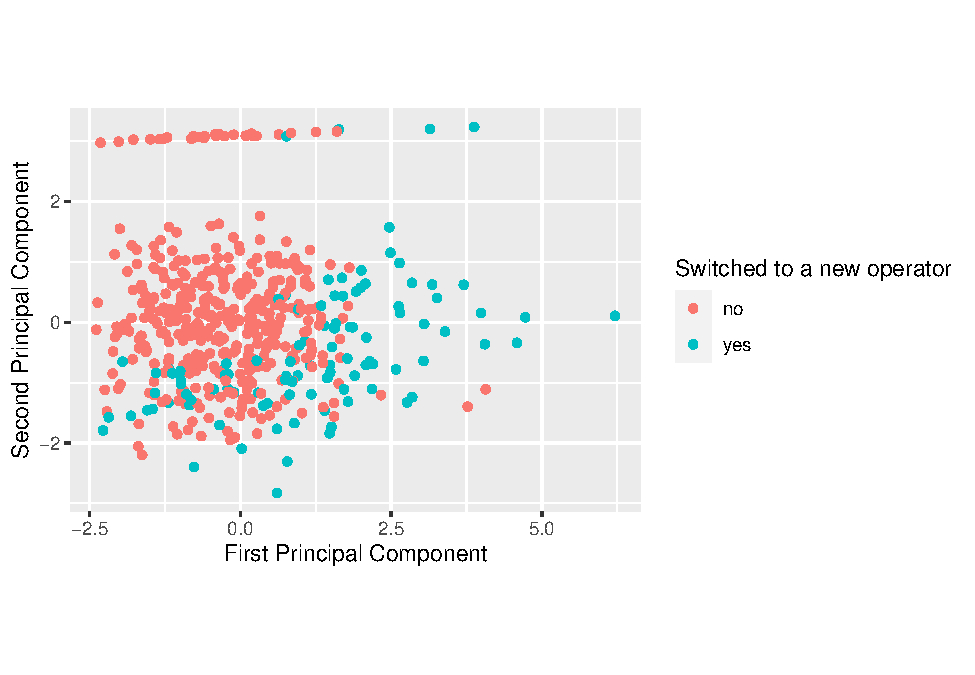
\includegraphics{Report_files/figure-latex/unnamed-chunk-30-1.pdf}

\textbf{What do you conclude?}

INSERT ANSWER HERE
\#\#\#\#\#\#\#\#\#\#\#\#\#\#\#\#\#\#\#\#\#\#\#\#\#\#\#\#\#\#\#\#\#\#\#\#\#\#\#\#\#\#\#\#\#\#\#\#\#\#\#\#\#\#\#\#\#\#\#\#

\end{document}
